�\chapter{PreProject}
\section{Rich Picture}

\begin{figure}[H]
 \begin{centering}
  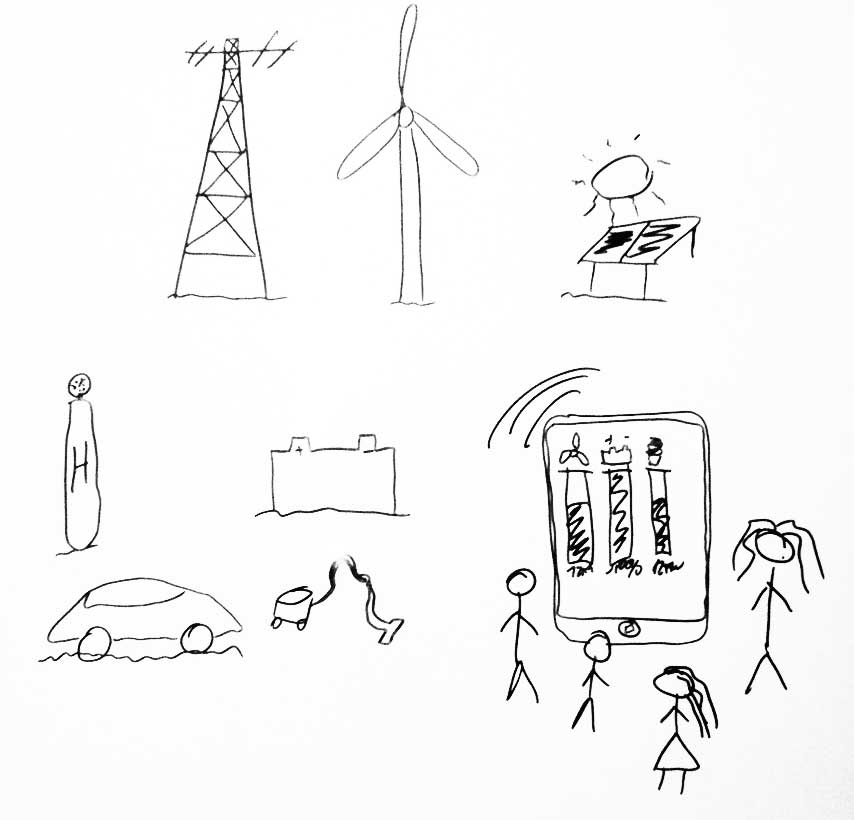
\includegraphics[width=0.7\textwidth]{images/rich_picture1.png}
   \caption{The surrounding environment is shown in the rich picture. The
 			 modules are: photovoltaic cells, CAES , battery-charger, wind-turbine
 			 converter, user-interface, the electric grid and different loads such as a
 			electric engine, vacuum-cleaner etc. }
 \end{centering}
\end{figure}

\section{Story Telling}
Jan Nielsen just got a new energy module to connect to his system. Luckily there is plenty of space
for new modules in the systems energy hub. He connects the device to the hub, where from the administrator web interface he can easily start the module.
The connection of the new modules is straight forward as all the module plugs are similar and the energy hub finds out by itself
if it is an input module, output module or both way module.
\p
Aarhus University - Herning, a place full of innovation and great ideas. Jan welcome a class of high-school students to the green system simulator. There
is possible to see the amount of energy that can be harvested in the green energy system
such as wind and solar energy. When the system produces to much energy, the 
energy is stored as compressed air. Here people can really come an get an idea about 
how much they can help the environment, but also their own finances, if they invest in green energy for their own house.
\p
Guests can interact with the system on a screen interface, they can see how much energy each module 
produces or consumes. This is shown in a intuitive manner, where everybody can follow, 
even persons without no special education or courses in the energy field.

\section{Story cards}
\textbf{Story Card 1:} Jan is looking at the web interface for the energy hub. From where he can see the status for each modules connected to it
in a graphically way.
\p
\textbf{Story Card 2:} A new energy module is connected to the hub, Jan opens the web interface for the energy hub, he logs in the administrator section of the system
to start, stop or see a more detailed overview of each module.
Jan really likes the graphically way that is also kept in the administrator section, this makes it possible for other
non-technically persons to operate the system if Jan is not there one day that the system needs to be operated.
\p
\textbf{Story Card 3:} It is one of many regularly autumn days in Denmark with rain and wind. The system is placed outside
but still it operates perfectly under these weather conditions. To operate the system or see the status for one of the modules,
it is not necessary for anyone to go outside to the module, they can simply log onto the system from their workstation pc or laptop.
\p
\textbf{Story Card 4:} Jan arrives at the university in the morning and an email was send to him reporting a failure in the green energy system, he login to the administrator web interface, and he can see what the problem might be, and if it's possible to solve it directly on the interface.
\p
\section{Preliminary Use Cases}

\begin{figure}[H]
	\begin{centering}
		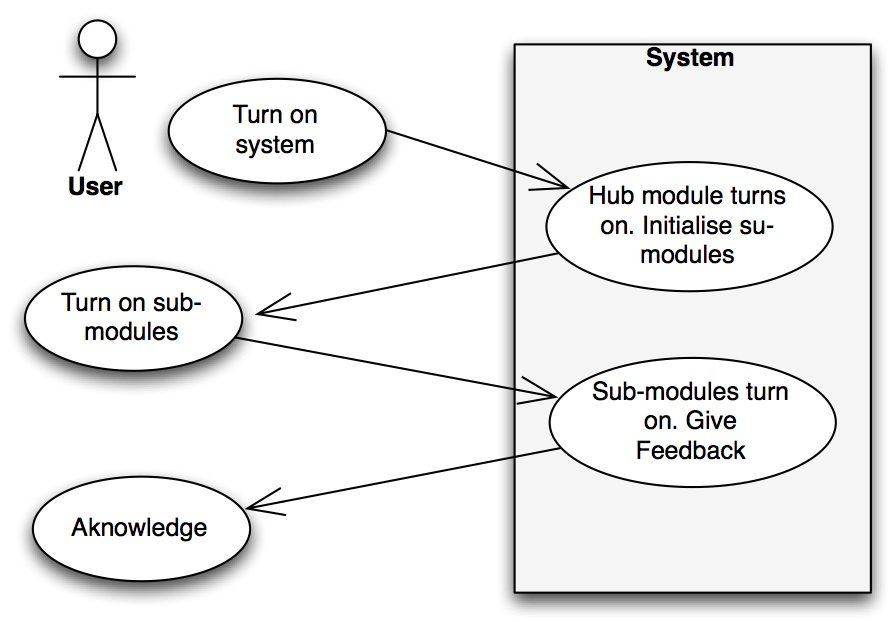
\includegraphics[width=0.7\textwidth]{images/usecases1.jpg}
		\caption{System initialization. }
	\end{centering}
\end{figure}

\begin{figure}[H]
	\begin{centering}
		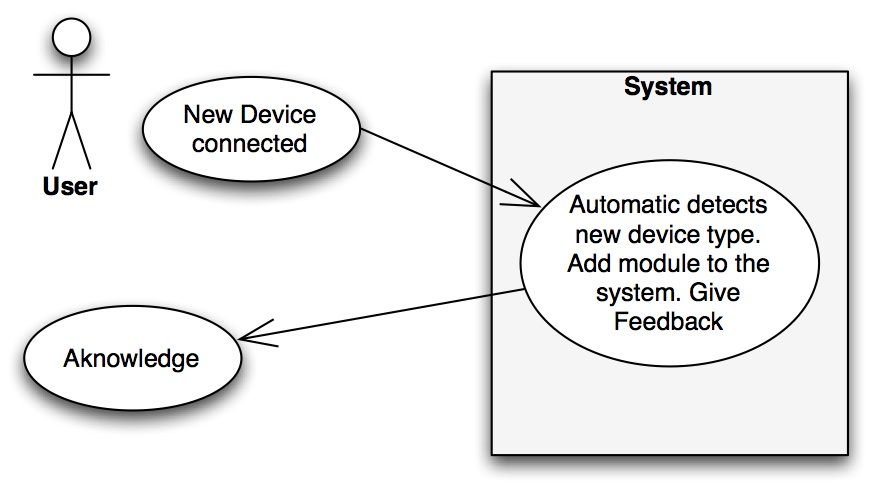
\includegraphics[width=0.7\textwidth]{images/usecases2.jpg}
		\caption{New device connected to the system. }
	\end{centering}
\end{figure}

\section{Stakeholder Analysis}

Stakeholder Analysis is an important tool for developers, as the different involvement of all person on the project and on the final product is clarified. This is done by identifying persons or groups which are relevant and their level of influence on the project.
\p
\textbf{Project coordinators:}\\ Morten Opprud\\ Klaus Kolle\\
\\
\textbf{Customers/Users:}\\
Jan Nielsen - Customer ( Primary User )\\
High school students ( Secondary Users )\\
Rene A. S. Josefsen ( Web interface customer )\\
\\
\textbf{Suppliers:}\\
Jens Mortensen\\
Per Lysgaard\\
\\
\textbf{Theory Advisors:}\\
Henning Slavensky\\
Ulrich Bjerre\\
Kristian Lomholdt\\
Per Lysgaard\\

\begin{figure}[h!]
 \begin{center}
  \begin{tabular}{| l | l | l |}
   \hline
    & \textbf{Has decision power} & \textbf{Has no decision power} \\ \hline
    \multirow{3}{*}{\textbf{Directly involved stakeholder}} 
    	& Klaus Kolle & Rene A. S. Josefsen\\ 
    	& Morten Opprud &  \\ 
    	& Jan Nielsen &  \\ \hline
    \multirow{2}{*}{\textbf{Not directly involved stakeholders}} 
    	&  & Jens Mortensen\\
    	& Per Lysgaard & High School Students \\ \hline
   \end{tabular}
  \end{center}
 \caption{Stakeholder Analysis table}
\end{figure}

Klaus Kolle and Morten Opprud, are the project coordinators/managers, they
have decision power over the final product and are directly involved on the development. As academic project, they are the persons that have to be satisfied with the final product. As project managers they guide the developers trough all the phases of the development process.\p

Jan Nielsen is the customer, the primary user of the system so he has the decision power over the final product and is enrol in all the development and design process. \p

Rene A. S. Josefsen is our web-interface customer, has no decision power in the overall system, but is direct involve in the design of the system interface.\p

In a real world project, Jan and Rene satisfaction as clients, would be very important. In this project their feedback is used as requirements for the final product.\p 

High School Students have no decision power over the final interface since they are the secondary users of the system. They will be one of the final users to test the system.\p

Jens Mortensen is the component supplier, is not directly involved in the project and has no decision power over the final product.\p

Per Lysgaard is not directly involved in the development of the system, but has the final decision of the budget for the system.\p

\section{System Definition}
\textbf{Proposal 1 - Fully automatically}\p
The Energy-Hub is the central device in the green-energy system. All
inputs and output devices are automatically routed inside this
device. When devices are connected to the Energy Hub, it automatically
detects if it's an input or an output module.\p
 On the web interface, the user have the possibility of using between two modes:
\\ - Green System profile.
\\ - Fast charging profile.
\\The Green profile only makes use of the green power devices such as
photovoltaic-cells, wind power, energy from the charged batteries or from the
compressed air module.
The fast charging profile on the other hand charges the compressed air module and the
battery directly from the grid.
\p
\textbf{Proposal 2 (Optimising):}\\
Extra output extension model: the user can connect devices, and switch
each output on and off. This module will be used to present to high school
students the interface navigation.





